\chapter{Learning From Data}

\section{Statistics}
Statistics is the science of learning from data. Statistical methods help us investigate questions in an objective manner. Statistical problem solving is an investigative process that involves four components: 

\begin{enumerate}
    \item formulate a statistical question
    \item collect data
    \item analyze data
    \item interpret results
\end{enumerate}

\subsection{Scenarios for Statistical Analysis}

\subsection*{Scenario 1: Predicting an Election Using an Exit Poll}

In elections, television networks often declare the winner well before all the votes have been counted. They do this using exit polling, interviewing voters after they leave the voting booth. Using an exit poll, a network can often predict the winner after learning how several thousand people voted, out of possibly millions of voters.

The 2010 California gubernatorial race pitted Democratic candidate Jerry Brown against Republican candidate Meg Whitman. A TV exit poll used to project the outcome reported that 53.1\% of a sample of 3889 voters said they had voted for Jerry Brown. Was this sufficient evidence to project Brown as the winner, even though information was available from such a small portion of the more than 9.5 million voters in California? We’ll learn how to answer that question in this book.

\subsection*{Scenario 2: Making Conclusions in Medical Research Studies}

Statistical reasoning is at the foundation of the analyses conducted in most medical research studies. Let’s consider three examples of how statistics can be relevant.

Heart disease is the most common cause of death in industrialized nations. In the United States and Canada, nearly 30\% of deaths yearly are due to heart disease, mainly heart attacks. Does regular aspirin intake reduce deaths from heart attacks? Harvard Medical School conducted a landmark study to investigate. The people participating in the study regularly took either an aspirin or a placebo (a pill with no active ingredient). Of those who took aspirin, 0.9\% had heart attacks during the study. Of those who took the placebo, 1.7\% had heart attacks, nearly twice as many.

Can you conclude that it’s beneficial for people to take aspirin regularly? Or, could the observed difference be explained by how it was decided which people would receive aspirin and which would receive the placebo? For instance, might those who took aspirin have had better results merely because they were healthier, on average, than those who took the placebo? Or, did those taking aspirin have a better diet or exercise more regularly, on average?

For years there has been controversy about whether regular intake of large doses of vitamin C is beneficial. Some studies have suggested that it is. But some scientists have criticized those studies’ designs, claiming that the subsequent statistical analysis was meaningless. How do we know when we can trust the statistical results in a medical study that is reported in the media?

\subsection*{Scenario 3: Using a Survey to Investigate People’s Beliefs}

How similar are your opinions and lifestyle to those of others? It’s easy to find out. Every other year, the National Opinion Research Center at the University of Chicago conducts the General Social Survey (GSS). This survey of a few thousand adult Americans provides data about the opinions and behaviors of the American public. You can use it to investigate how adult Americans answer a wide diversity of questions, such as, “Do you believe in life after death?” “Would you be willing to pay higher prices in order to protect the environment?” “How much TV do you watch per day?” and “How many sexual partners have you had in the past year?” Similar surveys occur in other countries, such as the Eurobarometer survey within the European Union. We’ll use data from such surveys to illustrate the proper application of statistical methods.

\subsection{The Statistical Method}

The scenarios just presented illustrate the three main components of statistics
for answering a statistical question:

\begin{enumerate}
    \item Design: Stating the goal and/or statistical question of interest and planning
how to obtain data that will address them
\item Description: Summarizing and analyzing the data that are obtained
\item Inference: Making decisions and predictions based on the data for answering
the statistical question
\end{enumerate}

\section{Sample Versus Population}

We’ve seen that statistics consists of methods for \textbf{designing} investigative studies, \textbf{describing} (summarizing) data obtained for those studies, and making \textbf{inferences} (decisions and predictions) based on those data to answer a statistical question of interest.

\subsection{We Observe Samples But Are Interested in Populations}

The entities that we measure in a study are called the \textit{subjects}. Usually subjects are people, such as the individuals interviewed in a General Social Survey. But they need not be. For instance, subjects could be schools, countries, or days. We might measure characteristics such as the following:
\begin{itemize}
    \item For each school: the per-student expenditure, the average class size, the average score of students on an achievement test
    \item For each country: the percentage of residents living in poverty, the birth rate, the percentage unemployed, the percentage who are computer literate
    \item For each day in an Internet café: the amount spent on coffee, the amount spent on food, the amount spent on Internet access
\end{itemize}

The \textbf{population} is the set of all the subjects of interest. In practice, we usually have data for only some of the subjects who belong to that population. These subjects are called a \textbf{sample}.

\subsection{Population and Sample}
The \textbf{population} is the total set of subjects/individuals in which we are interested. A \textbf{sample} is the subset of the population for whom we have (or plan to have) data, often randomly selected.

\subsection*{In Practice}

Sometimes the population is well-defined, but sometimes it is a hypothetical set of people that is not enumerated. For example, in a clinical trial testing the effectiveness of a new drug on lowering cholesterol, the population would be all people with high cholesterol who might have signed up for such a trial. This set of people is not specifically listed.

In the 2014 General Social Survey (GSS), the sample was the 2538 people who participated in this survey. The population was the set of all adult Americans at that time—more than 318 million people. 

Occasionally data are available from an entire population. For instance, every ten years the U.S. Bureau of the Census gathers data from the entire U.S. population (or nearly all). But the census is an exception. Usually, it is too costly and time-consuming to obtain data from an entire population. It is more practical to get data for a sample. The General Social Survey and polling organizations such as the Gallup poll usually select samples of about 1000 to 2500 Americans to learn about opinions and beliefs of the population of all Americans. The same is true for surveys in other parts of the world, such as the Eurobarometer in Europe.

\subsection{Descriptive Statistics and Inferential Statistics}

Using the distinction between samples and populations, we can now tell you more about the use of \textit{description} and \textit{inference} in statistical analyses.

\textbf{Descriptive statistics} refers to methods for summarizing the collected data (where the data constitutes either a sample or a population). The summaries usually consist of graphs and numbers such as averages and percentages.

A descriptive statistical analysis usually combines graphical and numerical summaries. For instance, Figure \ref{fig:education_levels.jpg} is a \textit{bar graph} that shows the percentages of educational attainment in the United States in 2013. It summarizes a survey of 78,000 households by the U.S. Bureau of the Census. The main purpose of descriptive statistics is to reduce the data to simple summaries without distorting or losing much information. Graphs and numbers such as percentages and averages are easier to comprehend than the entire set of data. It’s much easier to get a sense of the data by looking at Figure \ref{fig:education_levels.jpg} than by reading through the questionnaires filled out by the 78,000 sampled households. From this graph, it’s readily apparent that about a third of people have at least a bachelor’s degree, whereas about 11\% do not have a high school diploma.

\begin{figure}[h!]
\centering
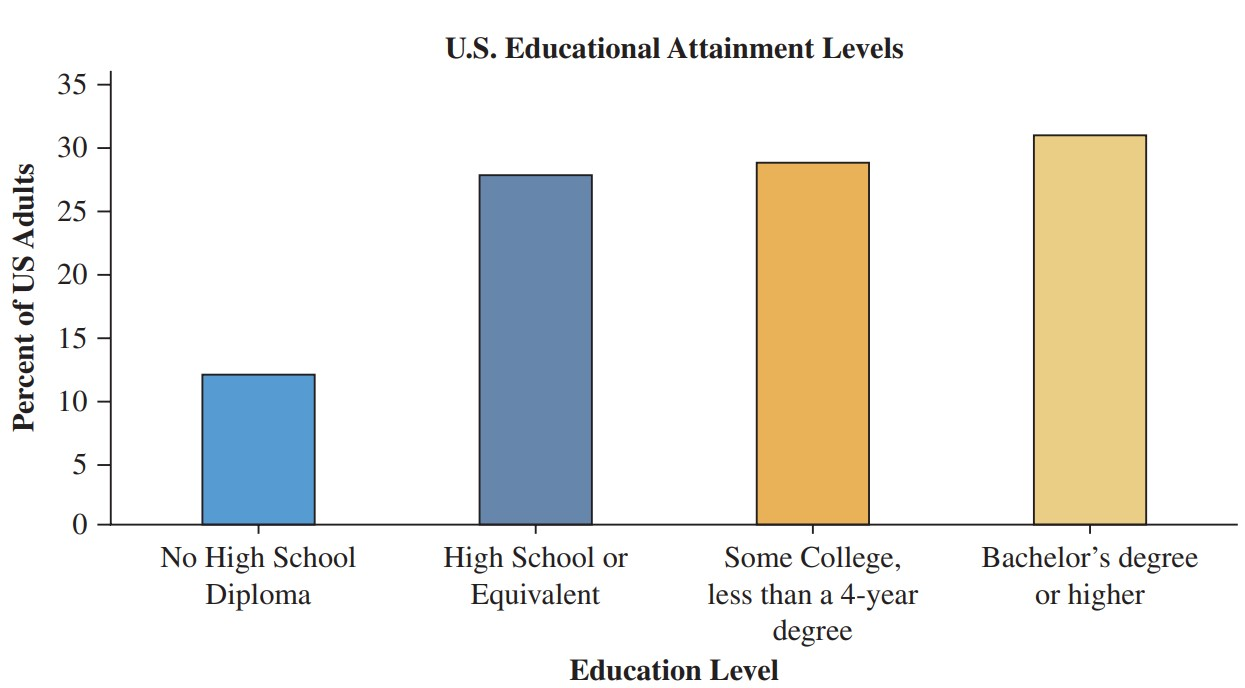
\includegraphics[width=0.8\textwidth]{figures/education_levels.jpg}
\caption{Educational Attainment, Based on a Sample of 78,000 Households in the 2013 Current Population Survey. (\textit{Source: Data from United States Census Bureau.})}
\label{fig:education_levels.jpg}
\end{figure}

Descriptive statistics are also useful when data are available for the entire population, such as in a census. By contrast, inferential statistics are used when data are available for a sample only, but we want to make a decision or prediction about the entire population.

\textbf{Inferential statistics} refers to methods of making decisions or predictions about a population, based on data obtained from a sample of that population.

In most surveys, we have data for a sample, not for the entire population. We use descriptive statistics to summarize the sample data and inferential statistics to make predictions about the population.

\subsection{Data, Individual, and Variable}
\begin{itemize}
    \item \textbf{Data} are numerical facts and figures from which conclusions can be drawn.
    \item \textbf{Individual:} The objects described by a set of data. Individuals may be people, but they may also be animals or things.
    \item \textbf{Variable:} Any characteristic of an individual. A variable can take different values for different individuals.
\end{itemize}

\subsection*{Types of Variables}
\begin{itemize}
    \item \textbf{Quantitative Variable:} Takes numerical values for which arithmetic operations such as adding and averaging make sense. The values of a quantitative variable are usually recorded with a unit of measurement (such as seconds or kilograms).
    \item \textbf{Categorical Variable:} Places an individual into one of several groups or categories. Categorical variables use labels. Example: gender.
\end{itemize}

\subsection*{Distribution of a Variable}
The distribution of a variable tells us what values the variable takes and how often it takes these values. The distribution of a categorical variable lists the categories and gives either the count or the percent of individuals who fall into each category.

\begin{table}[h!]
\centering
\begin{tabular}{|l|c|}
\hline
\textbf{Field of Study}             & \textbf{Percent of Students} \\ \hline
Arts and humanities                 & 10.6                         \\ \hline
Biological sciences                 & 14.7                         \\ \hline
Business                            & 14.5                         \\ \hline
Education                           & 5.2                          \\ \hline
Engineering                         & 11.2                         \\ \hline
Health professions                  & 12.8                         \\ \hline
Math and computer science           & 3.7                          \\ \hline
Physical sciences                   & 2.4                          \\ \hline
Social sciences                     & 10.1                         \\ \hline
Other majors and undeclared         & 14.9                         \\ \hline
\textbf{Total}                      & \textbf{100.1}               \\ \hline
\end{tabular}
\caption{Field of Study and Percent of Students}
\label{tab:field_of_study}
\end{table}


Table \ref{tab:field_of_study} contains data on the percents of first-year students who plan to major in several discipline areas.

\emph{Note:} The percentages for a categorical variable should add to 100\%, but oftentimes in practice we discover they add to something like 99.9\% or 100.1\%. This occurs sometimes when percentages are rounded. We call this \textbf{roundoff error}.

\subsection{Parameter and Statistic}
A \textbf{parameter} is a numerical summary of the population. A \textbf{statistic} is a numerical summary of a sample taken from the population.

\section{Solved Examples}

\paragraph{Example 1}
A professor collects information on students in her statistics course at University of Georgia. She records the students' majors, the number of books they read last semester, and whether or not they owned a pet (pet owner). In this context, “pet owner" is:
\begin{enumerate}[label=\alph*.]
    \item a categorical variable.
    \item a quantitative variable.
    \item not a variable.
    \item This can be interpreted as either a categorical variable or a quantitative variable based on the context in which it is used.
\end{enumerate}

\textbf{Correct Answer}: a categorical variable.

\paragraph{Example 2}
When ordering vinyl replacement windows, the following variables are specified for each window. Which of these variables is quantitative?
\begin{enumerate}[label=\alph*.]
    \item Window style—double-hung, casement, or awning.
    \item Area of the window opening, in square inches.
    \item Window style—single pane or double pane.
\end{enumerate}

\textbf{Correct Answer}: Area of the window opening, in square inches.

\paragraph{Example 3}
A professor collects information on students in her statistics course at University of Georgia. She records the students' majors, the number of books they read last semester, and whether or not they owned a pet. In this context, "number of books read" is:
\begin{enumerate}[label=\alph*.]
    \item a categorical variable.
    \item a quantitative variable.
    \item not a variable.
    \item This can be interpreted as either a categorical variable or a quantitative variable based on the context in which it is used.
\end{enumerate}

\textbf{Correct Answer}: a quantitative variable.

\paragraph{Example 4}
In a study of commuting patterns of people in a large metropolitan area, respondents were asked to report the time they took to travel to their place of work on a typical Monday morning. What is the variable of interest?
\begin{enumerate}[label=\alph*.]
    \item A person.
    \item City in which they lived.
    \item Travel time.
    \item Day of the week.
\end{enumerate}

\textbf{Correct Answer}: Travel time.

\paragraph{Example 5}
A political party's data bank includes the zip codes of past donors, such as those shown in the table. 

\begin{table}[h!]
\centering
\begin{tabular}{|c|c|c|c|c|c|c|c|}
\hline
47906 & 34236 & 53075 & 10010 & 90210 & 75204 & 30304 & 99709 \\ \hline
\end{tabular}
\caption{Data Row}
\label{tab:zip_code}
\end{table}

Zip code is a 

\begin{enumerate}[label=\alph*.]
    \item quantitative variable.
    \item unit of measurement.
    \item categorical variable.
\end{enumerate}

\textbf{Correct Answer}: categorical variable.

\section{Graphs for Categorical Variables}
The two primary graphical displays for summarizing a categorical variable are the \textbf{pie chart} and the \textbf{bar graph}.

A \textbf{pie chart} is a circle having a slice of the pie for each category. The size of a slice corresponds to the percentage of observations in the category.

A \textbf{bar graph} displays a vertical bar for each category. The height of the bar is the count or percentage of observations in the categories. The vertical bars for each category are apart, not side by side.

\subsection*{Shark Attacks in the United States}
For the United States alone, a total of 387 unprovoked shark attacks were reported between 2004 and 2013. Table \ref{tab:shark_attacks} shows the breakdown by state; states such as Oregon, Alabama, or Georgia with only a few attacks are summarized in the Other category.

\begin{table}[h!]
\centering
\begin{tabular}{|l|c|c|c|}
\hline
\textbf{U.S. State}      & \textbf{Frequency} & \textbf{Proportion} & \textbf{Percentage} \\ \hline
Florida                  & 203                & 0.525               & 52.5                \\ \hline
Hawaii                   & 51                 & 0.132               & 13.2                \\ \hline
South Carolina           & 34                 & 0.088               & 8.8                 \\ \hline
California               & 33                 & 0.085               & 8.5                 \\ \hline
North Carolina           & 23                 & 0.059               & 5.9                 \\ \hline
Texas                    & 16                 & 0.041               & 4.1                 \\ \hline
Other                    & 27                 & 0.070               & 7.0                 \\ \hline
\textbf{Total}           & \textbf{387}       & \textbf{1.000}      & \textbf{100.0}      \\ \hline
\end{tabular}
\caption{Unprovoked Shark Attacks in the U.S. Between 2004 and 2013 (\textit{Source: http://www.flmnh.ufl.edu/fish/sharks/statistics/statsus.htm.})}
\label{tab:shark_attacks}
\end{table}

\begin{figure}[h!]
\centering
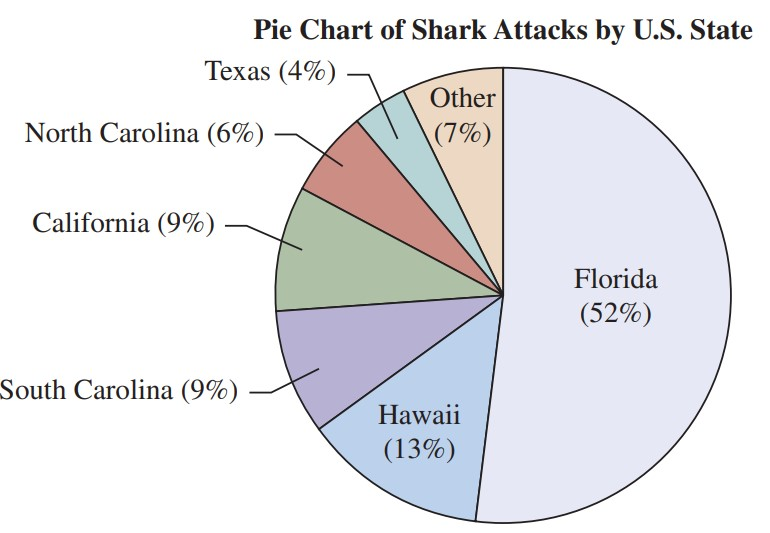
\includegraphics[width=0.6\textwidth]{figures/pie_chart.jpg}
\caption{Pie Chart of Shark Attacks Across U.S. States. The label for each slice of the pie gives the category and the percentage of attacks in a state. The slice that represents the percentage of attacks reported in Hawaii is 13\% of the total area of the pie.}
\label{fig:pie_chart.jpg}
\end{figure}

\begin{figure}[h!]
\centering
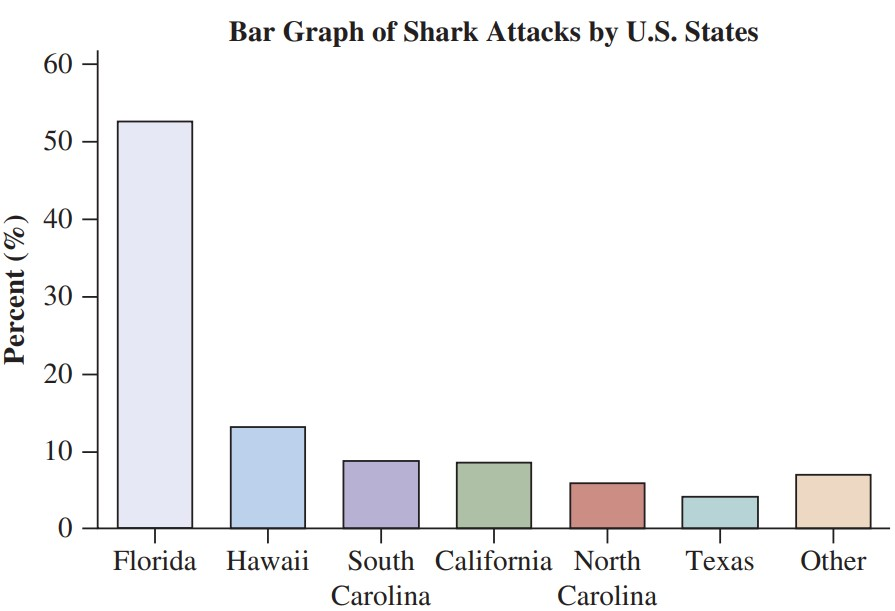
\includegraphics[width=0.6\textwidth]{figures/bar_chart.jpg}
\caption{Bar Graph of Shark Attacks Across U.S. States.}
\label{fig:bar_chart.jpg}
\end{figure}

\section{Graphs for Quantitative Variables}
We’ll look at three types of graphs for quantitative variables --- \textbf{dot plot}, \textbf{stem-and-leaf plot}, and \textbf{histogram}.

A \textbf{dot plot} shows a dot for each observation, placed just above the value on the number line for that observation.

\subsubsection*{How to Make a Dot Plot}
\begin{enumerate}
    \item Draw a horizontal line. Label it with the name of the variable and mark regular values of the variable on it.
    \item For each observation, place a dot above its value on the number line.
\end{enumerate}

Figure \ref{fig:dot_plot.jpg} gives an example of a \textbf{dot plot}.

\begin{figure}[h!]
\centering
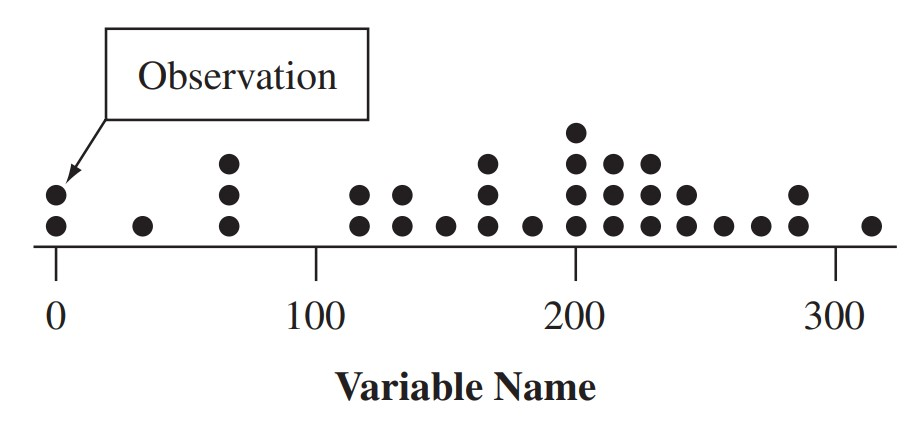
\includegraphics[width=0.6\textwidth]{figures/dot_plot.jpg}
\caption{An example of a dot plot.}
\label{fig:dot_plot.jpg}
\end{figure}

A \textbf{stem-and-leaf plot}, is similar to the dot plot in that it displays individual observations. Each observation is represented by a \textbf{stem} and a \textbf{leaf}.

\subsubsection*{How to Make a Stem-and-leaf plot}
\begin{enumerate}
    \item Separate each observation into a \textbf{stem} (consisting of all but the final/rightmost digit), and a \textbf{leaf} (the final/rightmost digit).
    \item Write the stems in a vertical column with the smallest at the top and draw a vertical line at the right of this column.
    \item Write each leaf in the row to the right of its stem, in increasing order out from the stem.
\end{enumerate}

Suppose we are given the data: 104, 105, 109, 110, 113, 113, 115, 127, 127, 127, 130, 136, 159. A \textbf{stem-and-leaf plot} will look like this:

\[
\begin{array}{c|l}
\textbf{Stem} & \textbf{Leaves} \\
\hline
10 & 4 \ 5 \ 9 \\
11 & 0 \ 3 \ 3 \ 5 \\
12 & 7 \ 7 \ 7 \\
13 & 0 \ 6 \\
14 & \\
15 & 9 \\
\end{array}
\]

\noindent The \textbf{stems} represent the tens digits, and the \textbf{leaves} represent the units digits of the numbers in the dataset.


A \textbf{histogram} is a graph that uses bars to display the frequencies or the relative frequencies of the possible outcomes for a quantitative variable. With a dot plot or a stem-and-leaf plot, it’s easy to reconstruct the original data set because the plot shows the individual observations. This becomes unwieldy for large data sets. In that case, a \textbf{histogram} is a more versatile way to graph the data and picture the distribution. 


\subsection*{TV Watching}
The 2012 General Social Survey asked, “On an average day, about how many
hours do you personally watch television?” Figure \ref{fig:histogram.jpg} shows the histogram of the 1298 responses. 

\begin{figure}[h!]
\centering
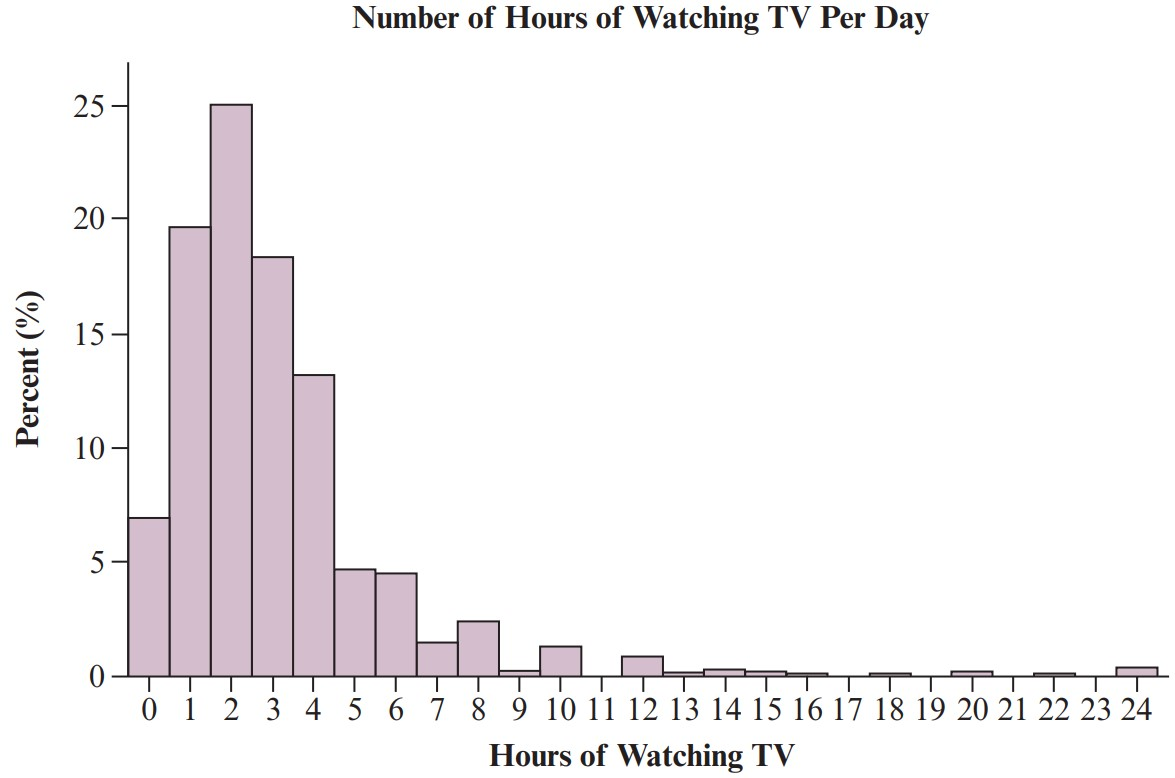
\includegraphics[width=0.8\textwidth]{figures/histogram.jpg}
\caption{Histogram of GSS Responses about Number of Hours Spent
Watching TV on an Average Day. (\textit{Source: Data from CSM, UC Berkeley})}
\label{fig:histogram.jpg}
\end{figure}

\section{Describing Shape of a Distribution}
A histogram (or a stem-and-leaf or dot plot) visualizes the distribution of a quantitative variable. If the distribution has a \textbf{single mound} or \textbf{peak}, the distribution is called \textbf{unimodal}, and the value that occurs most often is called the \textbf{mode}. A distribution with \textbf{two distinct mounds} is called \textbf{bimodal}. Figure \ref{fig:unimodal_bimodal.jpg} illustrates both a unimodal and a bimodal distribution.

A \textbf{bimodal} distribution can result when the observations come from two different groups. For instance, a histogram of the height of students at a school might show two peaks, one for females and one for males.

The shape of a \textbf{unimodal} distribution is often described as \textbf{symmetric}, or \textbf{skewed}. To \textbf{skew} means to stretch in one direction.

\begin{figure}[h!]
\centering
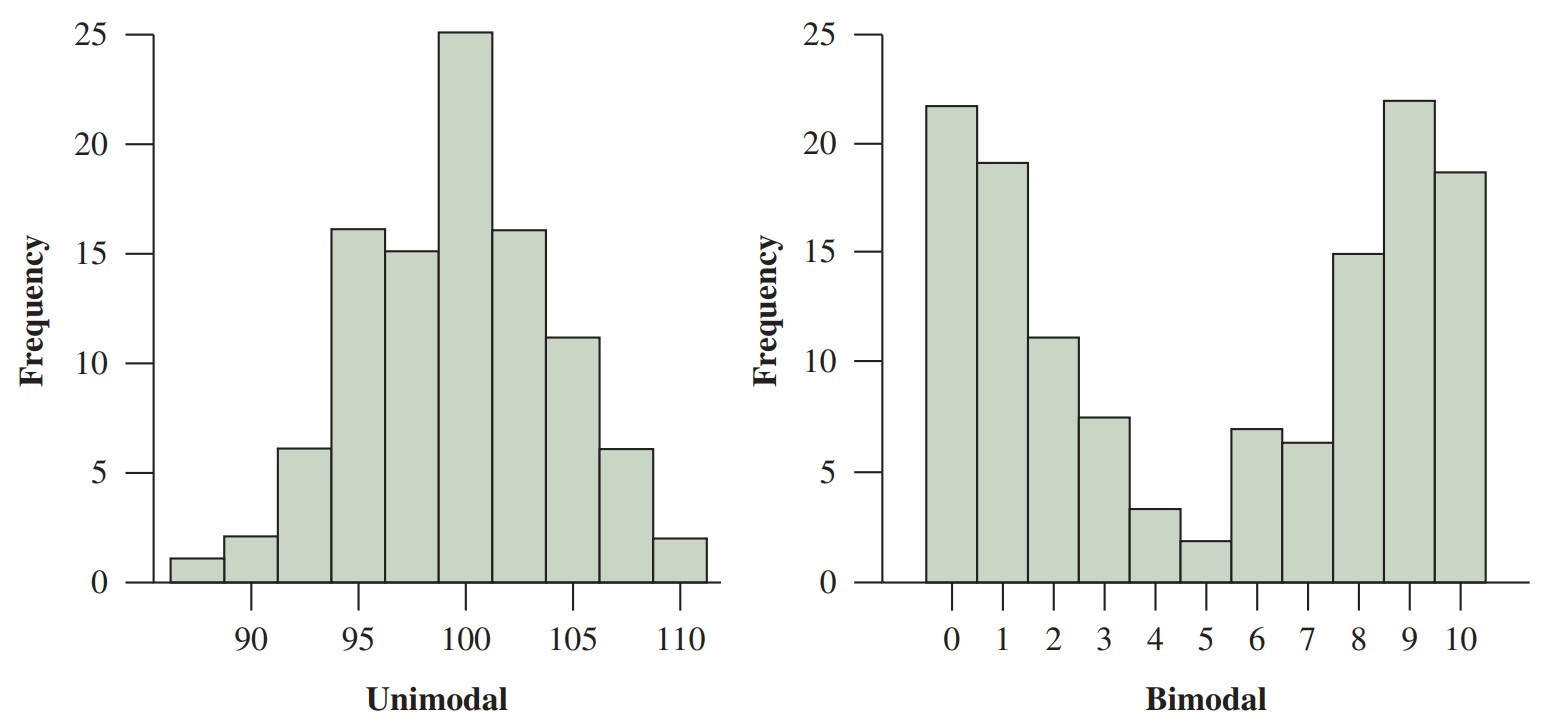
\includegraphics[width=1\textwidth]{figures/unimodal_bimodal.jpg}
\caption{Histograms of unimodal and bimodal distributions}
\label{fig:unimodal_bimodal.jpg}
\end{figure}

\subsection{Symmetric, or Skewed Distributions}

\begin{itemize}
    \item \textbf{Symmetric:} If the right and left sides of the distribution (histogram, stem-and-leaf plot, dot plot, or density curve) are approximately mirror images of each other.
    \item \textbf{Left-skewed:} If the distribution (histogram, stem-and-leaf plot, dot plot, or density curve) has a tail to the left direction.
    \item \textbf{Right-skewed:} If the distribution (histogram, stem-and-leaf plot, dot plot, or density curve) has a tail to the right direction.
\end{itemize}

Figure \ref{fig:shape.jpg} summarizes the shape of a unimodal distribution.

\begin{figure}[h!]
\centering
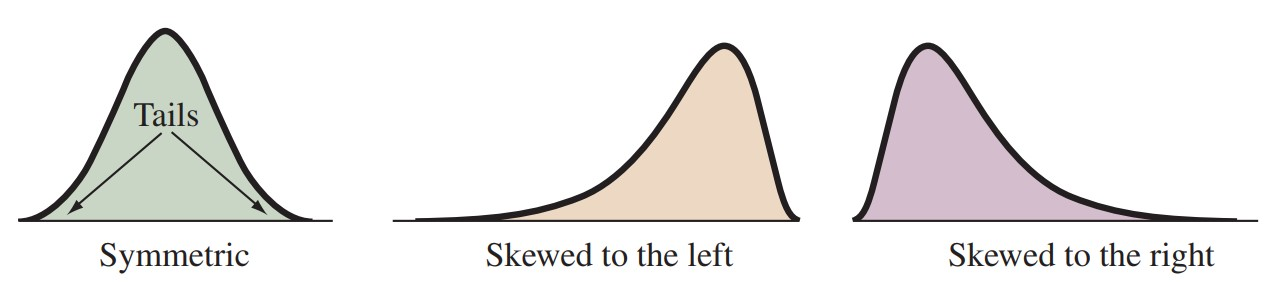
\includegraphics[width=1\textwidth]{figures/shape.jpg}
\caption{Curves for Distributions Illustrating Symmetry and Skew}
\label{fig:shape.jpg}
\end{figure}
